% !TEX root =  ../../thesis.tex 

\chapter{Bayesian paradigm}
\label{ch : bayesian_paradigm}
In this chapter we have introduced the basics of the Bayesian paradigm. i.e. Bayes rule and Bayesian summary measures. 

\section{The Bayesian motivation: A toy example}
What primarily differentiates the Bayesian paradigm from frequentist paradigm is that the parameters $\theta$ are random variables rather than being a constant. The distribution of parameters based on the data is called the posterior distribution and can be represented as $p(\theta|y)$. Whereas the initial distribution of parameters is called the prior distribution, represented by $p(\theta)$. To further signify the ideological differences between the Bayesian paradigm and frequentist paradigm we are presenting an example next.\\

Suppose there are three people A, B and C, of whom A and B each are captains of a sports team and C is the referee who tosses the coin. Let us assume that based on experiences of an old friend, captain B gets to know that the referee purposefully attempts at getting a heads on the toss. However given the nature of this problem, it is hard to quantify this belief in a single number. Instead a belief that there is a 70 to 90\% chance that the result will be a heads is more likely than a belief that there is exactly an 80\% chance for the same. One might also have a slightly vague belief that there is more than 50\% chance that the toss will result into a heads. Secondly, given the fact that not all coins are alike it is impossible for the probability of getting a heads to be constant, even if the referee tosses identically on each trial.\\

\begin{figure}
\centering
\captionsetup{justification=centering}
	\begin{subfigure}[b]{0.45\textwidth}
		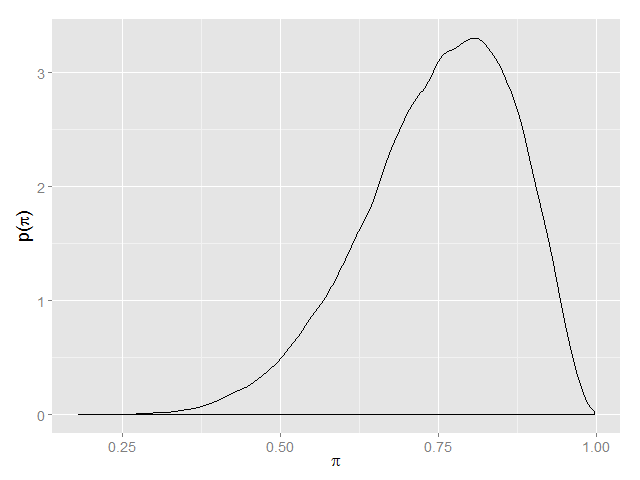
\includegraphics[width=\textwidth]{mainmatter/chapter_2_bayesian_paradigm/beta_prior.png}
        \caption{Prior $p(\pi)$: $\beta(9,3)$}
        \label{subfig : toy_problem_prior}
	\end{subfigure}
    	\begin{subfigure}[b]{0.45\textwidth}
		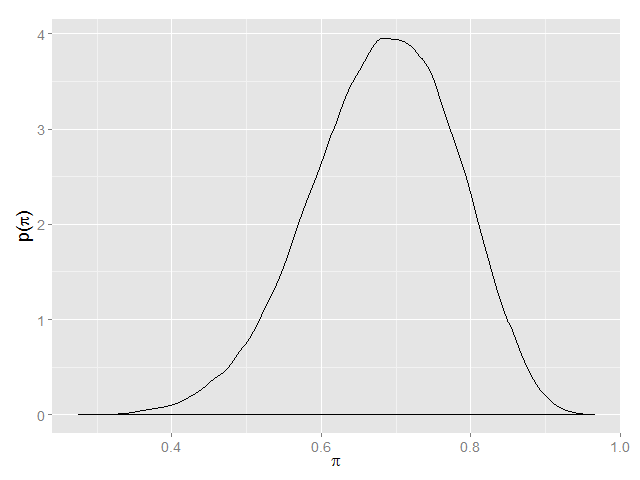
\includegraphics[width=\textwidth]{mainmatter/chapter_2_bayesian_paradigm/beta_posterior.png}
        \caption{Posterior $p(\pi|\boldsymbol{y})$: $\beta(15,7)$}
        \label{subfig : toy_problem_posterior}
	\end{subfigure}
\caption{Prior and posterior PDF for $\pi$; the probability of getting heads.}
\end{figure}

While the beliefs of captain B are subjective, they represent the prior probability distribution of a random variable in Bayesian paradigm. In our example the random variable is probability ($\pi$) of getting a heads. In figure \ref{subfig : toy_problem_prior} we can see one such prior distribution corresponding to the belief that the chance of getting a heads on the toss is more than getting tails and it is more likely to be somewhere between 70 to 90\%.

\section{Bayes rule}
\label{sec : bayes_rule}
We now present Bayes rule which is central to the Bayesian parameter estimation process. Bayes rule for the estimating the continuous parameter $\pi$ is given by

\begin{equation}
\label{eq : bayes_rule}
p(\pi|\boldsymbol{y}) = \dfrac{L(\pi|\boldsymbol{y})p(\pi)}{p(\boldsymbol{y})} = \dfrac{L(\pi|\boldsymbol{y})p(\pi)}{\int L(\pi|\boldsymbol{y})p(\pi)\diff\pi}
\end{equation}

The result $p(\pi|\boldsymbol{y})$ is called the posterior distribution of the parameter. It can be used to make statistical inference about the parameter $\pi$. An intuitive way to get the motivation behind the Bayes rule is to imagine the denominator as marginal probability of $\boldsymbol{y}$ calculated using the law of total probability.\\

It is also possible to apply Bayes rule for estimating parameters in context of the current example. Suppose after 10 matches captain B observed that 6 times out 10 the toss resulted in a heads. Assuming that the tosses were independent, then given the likelihood function $L(\pi|\boldsymbol{y})$, the MLE of $\pi$ will be $\hat{\pi} = 0.6$. Whereas Bayes rule gives us the entire posterior distribution of parameter $\pi$ as shown in figure \ref{subfig : toy_problem_posterior}. The mean value $E(p(\pi|\boldsymbol{y}))$ of the posterior distribution is 0.7, which if we compare with the MLE $\hat{\pi}$=0.6 we can see that Bayesian posterior mean is influenced by the prior as well.

\section{The role of prior distribution}
We can see in equation \ref{eq : bayes_rule} that the computation of posterior involves solving the integral in the denominator. One can avoid solving the integral by choosing a prior such that the resulting posterior is from the same parametric family as the prior and thus available in closed form. Such priors are termed as conjugate priors. However it is not always feasible to choose a conjugate prior and numerical approximation for calculation of the posterior is required. The most widely used algorithms for posterior approximation are Markov chain Monte Carlo (MCMC) techniques such as Gibbs sampling, Metropolis hastings algorithm, Hamiltonian Monte Carlo and their variants etc. The priors can also be classified as informative or non-informative/vague/diffuse. The prior we chose in our example was informative, whereas a diffuse prior could have been the uniform distribution $U(0,1)$. In absence of prior knowledge a non informative prior is advised. A more detailed overview of the priors can be found in \citet{lesaffre_bayesian_2012}.

\section{Bayesian inference}
Given the posterior distribution of a parameter $p(\theta|y)$ one can use the point estimates such as median, mean $E_\theta(\theta|y)$, or MAP (maximum a posteriori) $\argmax_\theta p(\theta|y)$ for inference. It is however the interval estimates where the Bayesian paradigm contrasts more with frequentist approach. Bayesian 95\% interval estimates are called credible intervals. While the frequentist 95\% confidence interval is interpreted as the interval in which 95 out of 100 times one can find the population parameter $\theta$, the Bayesian 95\% credible interval is interpreted as interval of the 95\% most plausible theta values a posteriori. The credible interval can be equal tailed or a highest posterior density interval (HPDI). The Bayesian paradigm also allows one to make inference on future values of the data by taking the current data into account. This is done using the posterior predictive distribution (PPD)

$$p(\tilde{y}|y) = \int p(\tilde{y}|\theta) p(\theta|y) \diff\theta$$

The point and interval summary measures for PPD are similar to the ones for posterior distribution of parameters $p(\theta|y)$. We will also discuss Bayesian model selection in the forthcoming chapters.

\section{Bayesian software}
Various Bayesian software tools such as BUGS, STAN, PROC MCMC in SAS etc. are used for running the MCMC procedures mentioned above. For the purpose of this thesis we used JAGS is strongly related to BUGS (Bayesian inference Using Gibbs Sampling) family. We also used the R package R2jags to execute JAGS code via R.